%%%% Paramétrage du TD %%%%
\def\xxactivite{Révisions \ifprof -- Corrigé \else \fi} % \normalsize \vspace{-.4cm}
\def\xxauteur{\textsl{Xavier Pessoles}}


\def\xxnumchapitre{Révision cinématique \vspace{.2cm}}
\def\xxchapitre{\hspace{.12cm} Résolution cinématique}
\def\xxonglet{\textsf{Rév -- Cin}}
\def\xxactivite{Application 03}
\def\xxauteur{\textsl{Xavier Pessoles}}

\def\xxpied{%
Révision cinématique \\
Fiche  2 -- \xxactivite%
}

\def\xxtitreexo{Étude des performances cinématiques en virage d’une Formule 1 \ifnormal $\star$ \else \fi \ifdifficile $\star\star$ \else \fi \iftdifficile $\star\star\star$ \else \fi}
\def\xxtitreexo{OMNIROB -- Le robot collaboratif de l'usine du futur d'Airbus}
\def\xxsourceexo{\hspace{.2cm} \footnotesize{ICNA 2019}}


\def\xxcompetences{%
\textsl{%
\textbf{Savoirs et compétences :}\\} \vspace{-.5cm}
%\begin{itemize}
%\item \textit{Res2.C18} : principe fondamental de la statique;
%\item \textit{Res2.C19} : équilibre d’un solide, d’un ensemble de solides;
%\item \textit{Res2.C20} : théorème des actions réciproques.
%\end{itemize}
}


\def\xxfigures{
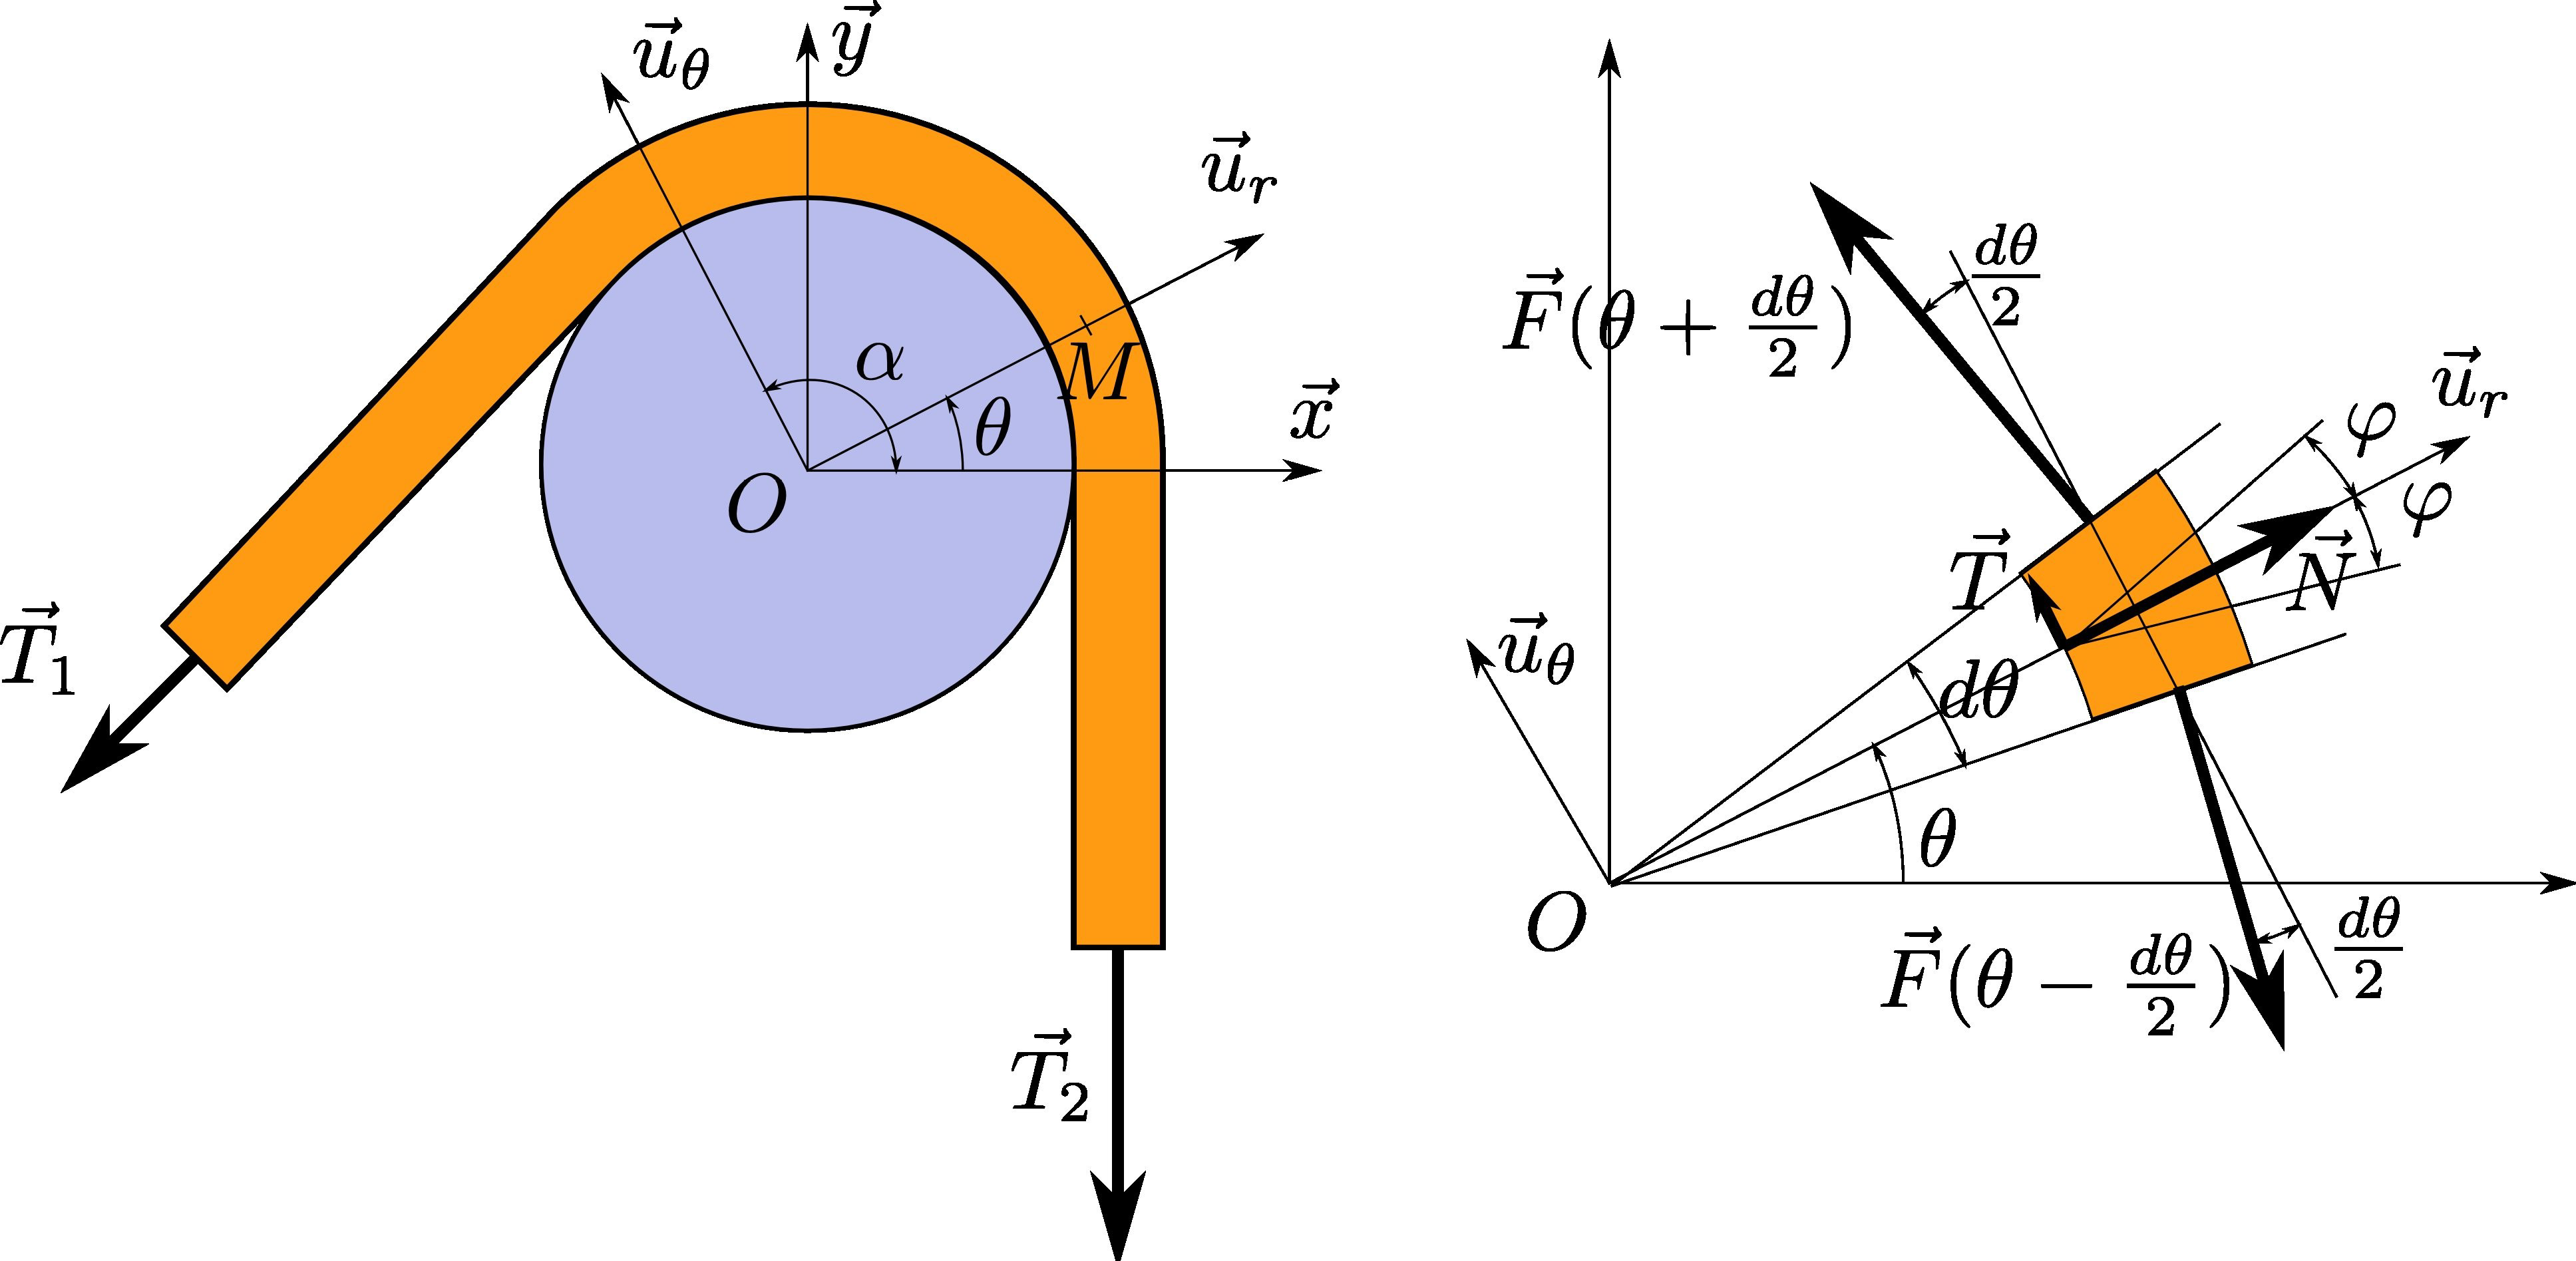
\includegraphics[width=.6\textwidth]{fig_01}
}%figues de la page de garde




\iflivret
\input{../../style/new_pagegarde}
\else
\input{../../style/new_pagegarde}
\fi
\setlength{\columnseprule}{.1pt}

\pagestyle{fancy}
\thispagestyle{plain}

\ifprof
\vspace{5cm}
\else
\vspace{4cm}
\fi

\def\columnseprulecolor{\color{ocre}}
\setlength{\columnseprule}{0.4pt} 

%%%%%%%%%%%%%%%%%%%%%%%

\setcounter{exo}{0}


\ifprof
\else
\begin{multicols}{2}
\fi

\begin{obj}
Déterminer le modèle cinématique direct ou inverse de la commande Omnirob. 

Valider le critère de mobilité omnidirectionnelle et analyser les limites du modèle.
\end{obj}


Les roues utilisés pour le robot omnirob sont des roues holonomes  également appelées Mecanum (voir figure suivante) qui sont mises en mouvement par quatre moteurs commandés indépendamment. La surface de roulement de ces roues spéciales est pourvue de rouleaux ellipsoïdes répartis sur la circonférence à un angle de 45\degres. 



\begin{center}
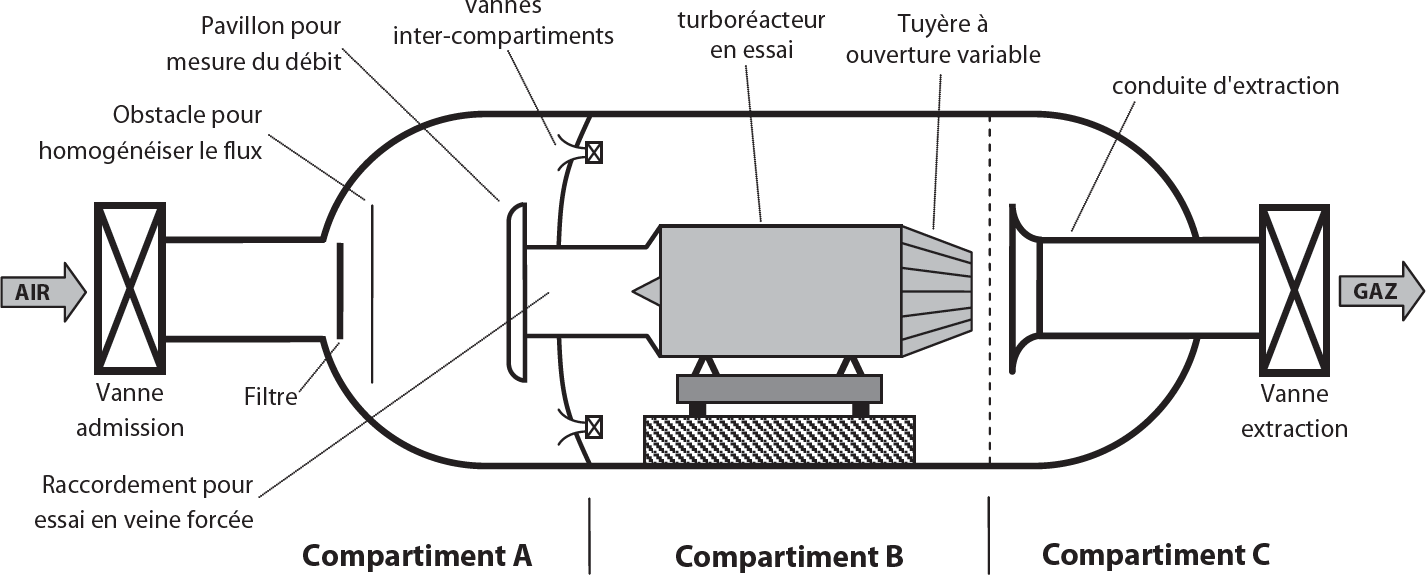
\includegraphics[width=\linewidth]{fig_02}
%\textit{}
\end{center}


Le paramétrage cinématique est donné dans les pages suivantes. 

\subparagraph{}
\textit{En analysant la géométrie du contact entre les rouleaux et le sol, proposer la liaison équivalente entre le châssis 3 et le sol.}
\ifprof%
\begin{corrige}
\end{corrige}\else\fi

Hypothèses : 
\begin{itemize}
\item Les roue sont parfaitement symétriques par rapport aux plans $\left(O_3,\vect{x_3},\vect{z_3}\right)$
et $\left(O_3,\vect{y_3},\vect{z_3}\right)$.
\item Les roues roulent sans glisser sur le sol.
\end{itemize}

Données : 
\begin{itemize}
\item Le nombre de rouleaux \textbf{1} par roue est $n=8$. 
\item Les rouleaux sont inclinés d'un angle $\alpha_a=-45\degres$ par rapport à l'axe de rotation de la roue.
\end{itemize}

Notations : torseurs cinématiques.
\begin{itemize}
\item Le torseur cinématique de 3/0 pourra s'exprimer dans la base locale du robot $\mathcal{B}_3 = \base{x_3}{y_3}{z_3}$ avec les notations $\torseurcin{V}{3}{0} = \torseurl{\vecto{3}{0}}{\vectv{O_3}{3}{0}}{O_3}$
$\torseurl{\dot{\varphi}\vect{z_3}=\omega \vect{z_3}}{V_{RX}\vect{x_3}+V_{RY}\vect{y_3}}{O_3}$.
\end{itemize}

Dans le mouvement de rotation de la roue a, le rouleau 1 reste en contact avec le sol suivant la corde 
$I_{1a\_\text{ext}}I_{1a\_\text{int}}$ (annexe 4).


On peut alors démontrer que la fluctuation du rayon $r$ de l'ellipsoïde est telle que : $\Delta r_{\%} = \left( \dfrac{1-\cos\dfrac{\pi}{n}}{\sin \dfrac{\pi }{n}}\right)\sin \alpha_a$ avec $n$ le nombre de rouleaux. 


Pour les roues de cette étude, $\alpha_a=-45\degres$ et $n=8$ rouleaux, on obtient une fluctuation de rayon de \SI{14}{\%} lorsque le point de contact $I_{1a}$ se déplace le long de la corde de rouleau 1. On supposera donc le rayon $r$ comme étant constant. 

\subparagraph{}
\textit{Déterminer $\vectv{I_{1a}}{1}{2}$ en fonction du paramétrage du robot dans la base $\mathcal{B}_3$.}
\ifprof%
\begin{corrige}
\end{corrige}\else\fi

On constate que la variation d'angle $\theta_{2a}$ lors du contact d'un rouleau avec le sol reste faible, 
$\theta_{2a} << 1$. Ainsi, en effectuant un développement limité à l'ordre 1 de $\cos \theta_{2a}$, on gardera pour la suite du sujet une expression de la vitesse $\vectv{I_{1a}}{1}{2}=r\dfrac{\sqrt{2}}{2}\dot{\theta}_{1a} \begin{pmatrix}
1 \\ 1 \\ 0 \end{pmatrix}_{\mathcal{B}_3}$


\subparagraph{}
\textit{En vous aidant de l'annexe 3, déterminer $\vectv{I_{1a}}{2}{3}$ en fonction du paramétrage du robot.}
\ifprof%
\begin{corrige}
\end{corrige}\else\fi

\subparagraph{}
\textit{En vous aidant de l'annexe 1, déterminer $\vectv{I_{1a}}{3}{0}$ en fonction du paramétrage du robot et des notations du torseur cinématique $\torseurcin{V}{3}{0}$ proposées.}
\ifprof%
\begin{corrige}
\end{corrige}\else\fi

\subparagraph{}
\textit{Déterminer $\vectg{I_{1a}}{3}{0}$.}
\ifprof%
\begin{corrige}
\end{corrige}\else\fi


Afin d'établir le modèle cinématique du robot, on introduit une notation classique en robotique avec les vecteurs suivants :
 \begin{itemize}
\item  $\dot{q}_k$ étant le vecteur des vitesses articulaires des roues $k=a,b,c$ et $d$ tel que $\dot{q}_k =\begin{pmatrix}
\dot{\theta}_{2k} \\ \dot{\theta}_{1k} \\ \dot{\varphi} \end{pmatrix} $ $=\begin{pmatrix}
\omega_{2k} \\ \omega_{1k} \\ \omega \end{pmatrix} $. On aura par exemple pour la roue $a$ le vecteur 
$\dot{q}_a =\begin{pmatrix}
\omega_{2a} \\ \omega_{1a} \\ \omega \end{pmatrix} $.
\item  $\dot{q}$ étant le vecteur des vitesses articulaires pilotées donc les vitesses des 4 moteurs des roues $a$, $b$, $c$ et $d$ tel que $\dot{q} =\begin{pmatrix}
\omega_{2a} \\ \omega_{2b}\\ \omega_{2c}\\ \omega_{2d}\end{pmatrix} $;
\item $\dot{X}_R$ étant le vecteur des vitesses opérationnelles du robot tel que $\dot{X}_R=\begin{pmatrix}
V_{RX} \\ V_{RY}\\ \dot{\varphi}\end{pmatrix} $ $=\begin{pmatrix}
V_{RX} \\ V_{RY}\\ \omega\end{pmatrix} $ exprimé dans la base locale $\mathcal{B}_3$ du robot.
 \end{itemize}


Dans un premier temps nous allons chercher les relations entre $\dot{X}_R = f\left(\dot{q}_k \right)$ pour 
$k=a$, $b$, $c$ et $d$.

\subparagraph{}
\textit{À partir des équations des questions 2 à 4, déduire de la condition de roulement sans glissement du rouleau 1 par rapport au sol 0 la relation $\dot{X}_R = f\left(\dot{q}_k \right)$  pour la roue $a$. On utilisera les notations proposées e ton rappelle que l'on note $\omega=\dot{\varphi}$.}
\ifprof%
\begin{corrige}
\end{corrige}\else\fi

La relation précédente pourra se noter $\dot{X}_R = \mathcal{I}_a \begin{pmatrix}
\omega_{2a} \\ \omega_{1a}\\ \omega_{}\end{pmatrix}$ avec $\mathcal{I}_a$ la matrice jacobienne relative à la roue $a$.

De façon analogue en prenant $\lambda$, $-\lambda$, $\ell$ ou $-\ell$ on trouve rapidement les matrices jacobiennes relatives aux roue $b$, $c$ et $d$.

$\dot{X}_R$ étant unique on peut obtenir 4 équations faisant intervenir uniquement les 4 inconnues articulaires $\omega_{2a}$, $\omega_{2b}$, $\omega_{2c}$ et $\omega_{2d}$que l'on souhaite déterminer.

En effet, pour chaque relation $\dot{X}_R = f\left(\dot{q}_k \right)$ on peut écrire pour :
\begin{itemize}
\item la roue $a$ : $V_{RX}-V_{RY}=R\omega_{2a}+\left(\lambda+\ell\right)\omega$ (eq1);
\item la roue $b$ : $V_{RX}+V_{RY}=-R\omega_{2b}+\left(\lambda+\ell\right)\omega$ (eq2);
\item la roue $c$ : $V_{RX}-V_{RY}=R\omega_{2c}-\left(\lambda+\ell\right)\omega$ (eq3);
\item la roue $d$ : $V_{RX}+V_{RY}=-R\omega_{2d}-\left(\lambda+\ell\right)\omega$ (eq4).
\end{itemize}

Trouver le modèle cinématique direct (MCD) revient à obtenir $\dot{X}_R = f\left(\dot{q}_k \right)$. Ainsi on remarquera que les coordonnées de $\dot{X}_R$ se déduisent facilement en utilisant les simplifications issues des 3 combinaisons :
\begin{itemize}
 \item (eq1)+(eq2)+(eq3)+(eq4);
 \item (eq2)-(eq1)+(eq4)-(eq3);
 \item (eq1)+(eq2)-(eq3)-(eq4).
\end{itemize}



\subparagraph{}
\textit{Déduire de ces 3 simplifications, le modèle cinématique direct (MCD) du robot, $\dot{X}_R = f\left(\dot{q}_k \right)$.}
\ifprof%
\begin{corrige}
\end{corrige}\else\fi

\subparagraph{}
\textit{Déduire également à l'aide des équations (eq1), (eq2), (eq3), (eq4), le modèle cinématique inverse (MCI) du robot 
$\dot{X}_R = f\left(\dot{q}_k \right)$.}
\ifprof%
\begin{corrige}
\end{corrige}\else\fi




Le contrôle du robot peut également être envisagé dans l'espace de travail lié au bâti à savoir le système de coordonnées du repère global.

En notant $\torseurcin{V}{3}{0}= \torseurl{\vecto{3}{0}}{\vectv{O_3}{3}{0}}{O_3}$ 
$\torseurl{\dot{\varphi}\vect{z_0}=\omega\vect{z_0}}{V_X\vect{x_0}+V_Y\vect{y_0}}{O_3}$ 
le torseur cinématique de 3/0 dans la base $\mathcal{B}_0=\base{x_0}{y_0}{z_0}$,
le changement de base étant une rotation d'un angle $\varphi$ selon $\vect{z_0}$, il vient immédiatement

$$
\begin{pmatrix} V_{RX} \\ V_{RY} \\ \omega \end{pmatrix}
=
\begin{bmatrix}  
\cos \varphi  &  \sin \varphi & 0 \\
- \sin \varphi & \cos \varphi & 0 \\
0 &  0 & 1 \\
\end{bmatrix}
\begin{pmatrix}
V_X \\ V_Y \\ \omega
\end{pmatrix}.
$$

\subparagraph{}
\textit{À partir des résultats précédents, indiquer comment commander la vitesse de rotation des moteurs des 4 roues $a$, $b$, $c$ et $d$ pour que le robot se déplace suivant une direction diagonale puis tourne sur lui-même, $\omega_m$ est une vitesse de rotation algébrique.}
\ifprof%
\begin{corrige}
\end{corrige}\else\fi

\begin{center}
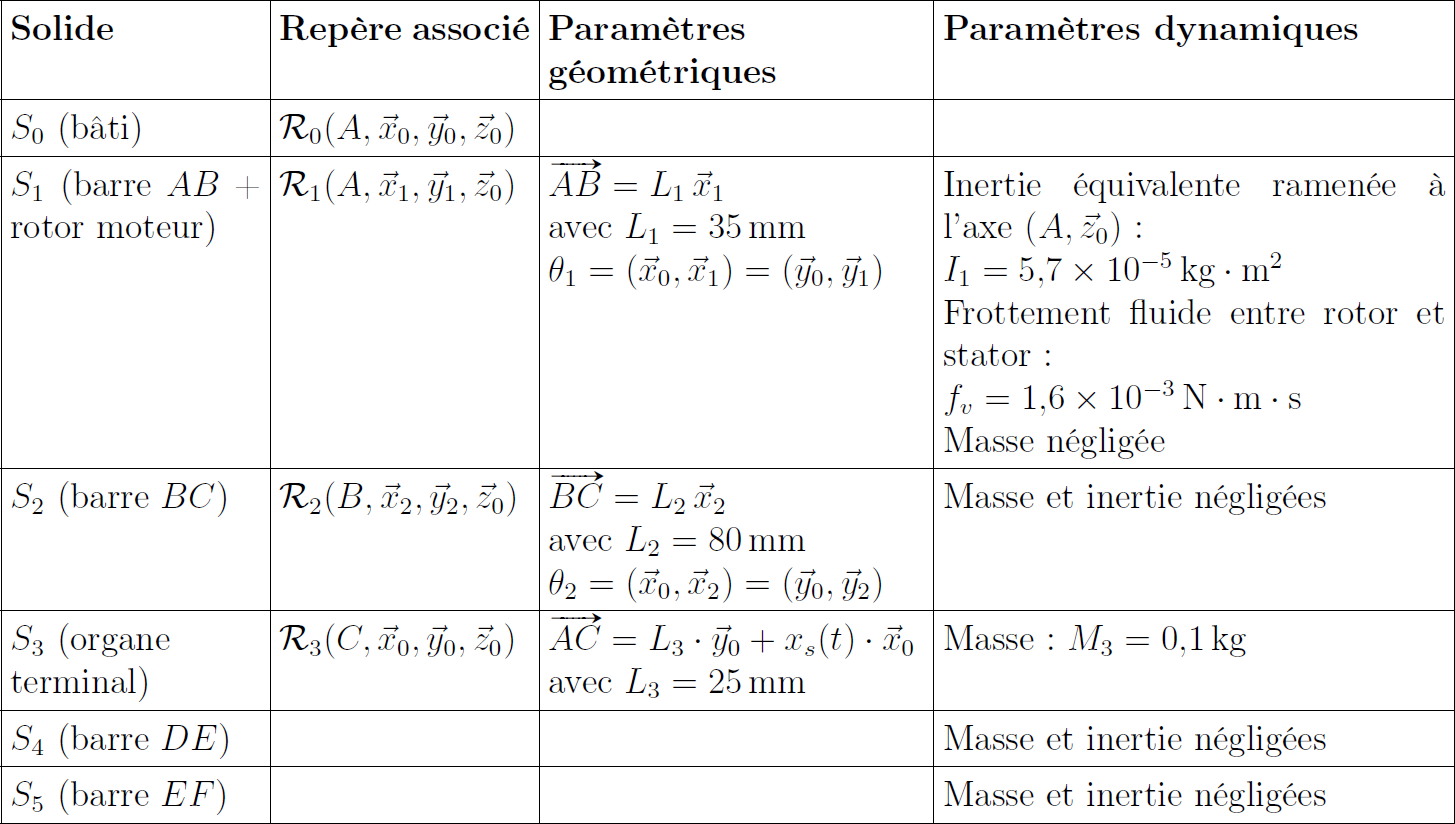
\includegraphics[width=\linewidth]{fig_07}
\end{center}



\subparagraph{}
\textit{Conclure sur le comportement omnidirectionnel du robot des limites possibles.}
\ifprof%
\begin{corrige}
\end{corrige}\else\fi

\ifprof
\else
\end{multicols}
\fi


\begin{center}
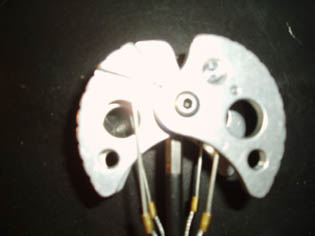
\includegraphics[width=\linewidth]{fig_03}

\textit{Annexe 1 : Schéma cinématique plan du robot -- Paramétrages repères robot et repère global}
\end{center}
\begin{center}
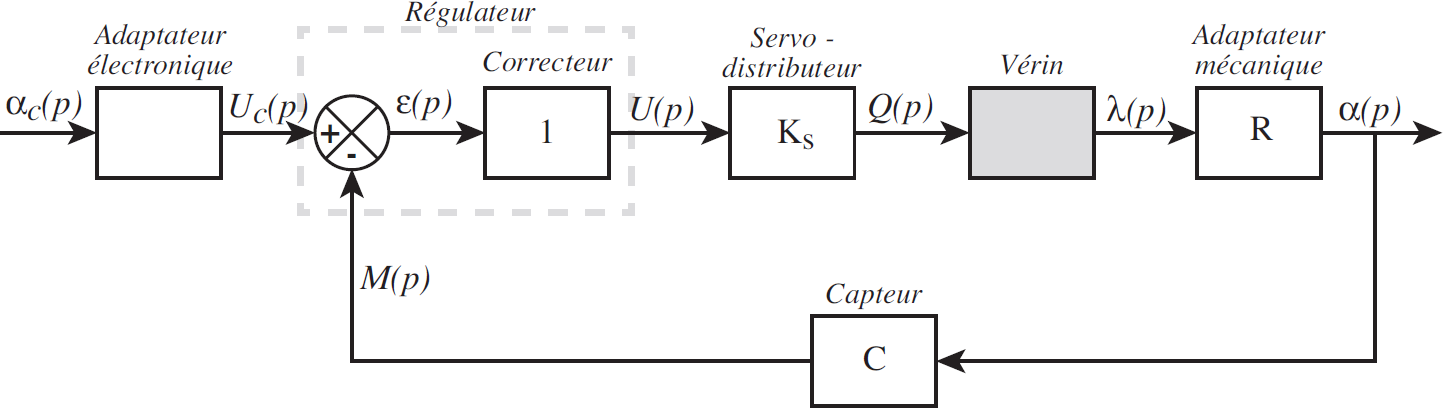
\includegraphics[width=\linewidth]{fig_04}

\textit{Annexe 2 : Schéma cinématique 3D de principe du robot -- Représentation partielle du châssis 3 avec la roue a}
\end{center}
\begin{center}
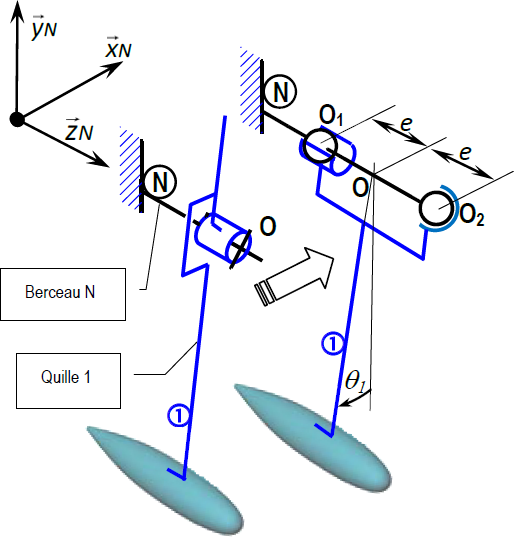
\includegraphics[width=\linewidth]{fig_05}

\textit{Annexe 3 : Schéma cinématique de la roue a dans le plan vertical contenant l'axe de la jante 2 soit $\left( O_{3a},\vect{y_3},\vect{z_3}\right)$}
\end{center}
\begin{center}
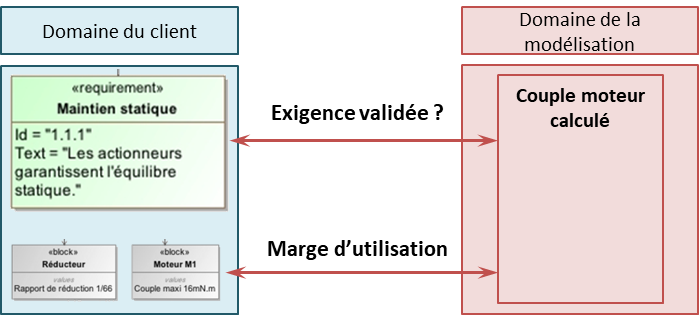
\includegraphics[width=\linewidth]{fig_06}

\textit{Annexe 4 : Schéma cinématique partiel du rouleau 1 seul de la roue a dans la position particulière où $I_{1a}$ se trouve au milieu de l'arc $I_{1a\_\text{ext}}I_{1a\_\text{int}}$.}

\end{center}
